Being some of the decoder's behaviors created, the next step was the implementation of the conceptual model of the \textit{DBT} using the \textit{EL} language. This task was performed by all elements of the groups dedicated to this model, although, each group was responsible for creating the files for the specific components. After, the source files were  annotated and the elaboration files were created as will be shown in this chapter.

\subsubsection{EL scripts}

\subsubsubsection*{Language}
The first step was the declaration of the \textbf{language}. The original code was developed in C++, therefore, an entity called \texttt{Cplusplus} was crated in a file named \texttt{Languages.el} (listing \ref{lst:EL_DBT_language}). This elements contains as attribute the symbols used to limit the annotation placed in the source files. In this case, the symbol chosen was \texttt{\@\@}.


\begin{lstlisting} [language=EL, caption=Language (EL representation).
, label=lst:EL_DBT_language]
language cpp
{
		annotation: "@@"
}
\end{lstlisting}

\subsubsubsection*{Interfaces}
After the declaration of the language, the several \textbf{interfaces} established were defined in a file called \texttt{Interfaces.el} (listing \ref{lst:EL_DBT_interfaces}). The methods inside each interface were already explained in the design chapter.

\begin{lstlisting} [language=EL, caption=Interfaces (EL representation).
, label=lst:EL_DBT_interfaces]
// Source & Target Architecture components 
interface i_ISA {   //Instruction Set 
		getWordSize	
		PCSize
		nBitsOpcode }
    
interface i_MemSizes{  //Memory of architecture
		xDataMemSize  DataMemSize 	
		MemSize	HeapSize StackSize  }

interface i_Registers {	 }  //Registers of architecture 

// SourceEnvironment 
interface i_SrcEnv {   
		getPC  setPC
		envReset  }

// TCache 
interface i_TCache {  //read/write and management operations
		addTag 	cacheCode			
		getTransAddr  getLastTransAddr  getCurrInsAddr  }

// CCache 
interface i_CCache {     //read operation and initialization
		fetch  load    }

// DATA MEMORY 
interface i_DMem {    //Data memory access
		readDataMem   writeDataMem	}

// DECODE 
interface i_Decode {    //decode service
		decode   }

//GENERATOR 
interface i_Generate {   //gen functions
		...
		gen_helper	gen_brkp  	gen_blx    gen_PUSH  	gen_POP
		gen_cmp 	gen_cmpi   gen_it   gen_mov  	gen_movi
		gen_cje  	gen_cjne	gen_cjei  	gen_cjnei
		gen_writePC gen_writePCreg   gen_ld8  	gen_ld16  gen_ldi8
		gen_st8	 	gen_st16  gen_sti8  gen_ld_bit  gen_st_bit
		gen_add  	gen_addi  gen_sub  	gen_subi  gen_div  
		gen_mul     gen_or  gen_ori   gen_not
		gen_and  	gen_andi    gen_xor  gen_shri 	gen_shli
		gen_orShl   gen_prolog gen_epilog
        ... }
    
// TRANSLATOR
interface i_Translate {   //Tanslate service
		translate }

// EXECUTOR 
interface i_Execute{
		execute
}

// DBTEngine 
interface i_CurrBBExec {   
		currBBExecPtr	}

interface i_Engine{
		initTranslator		runDBT  }

interface i_EngineState{
		eoBB  eoExec   pSourceProgMem  }
\end{lstlisting}


\subsubsubsection*{DBT Component}

Finally, the \textit{EL} representation of the components was created.  Each components was declared in a separated \texttt{.el} file. Given the amount of components in the model, only two \textit{EL} files will be shown: the \textbf{DBT} component, defined as a top level, and the \textbf{Decoder}, the component which responsibility relies on the group. Since several behaviors where created, the Decoder is explained in the following section. The \texttt{.el} files of the other components are presented in appendix. Listing \ref{lst:EL_DBT_component} shows the \textit{DBT} component coded using the \textit{EL} language.


\begin{lstlisting} [language=EL, caption=DBT component (EL representation), label=lst:EL_DBT_component]
import "Languages.el"
import "Interfaces.el"
import "Architectures.el" //Source and Target Architectures 
import "SourceCluster.el" // Source Group
import "TargetCluster.el" // Target Group 
import "DBTEngine.el" // DBT Engine
import "CodeCache.el" // Memory Structures 
import "TranslationCache.el"   //Translation Cache
import "DataMemory.el"   //DataMemory 

compile DBT   //top level component to be compiled
component DBT (C){
	properties:
		bool Measure : true
		
	subcomponents:
		SourceCluster srcCluster
		TargetCluster trgCluster
		CodeCache cCache
		TranslationCache tCache	
		DBTEngine dbtEngine
		
	references:
		i_Engine r_Engine
		i_MemSizes r_TrgMemSizes
		i_MemSizes r_SrcMemSizes
		
	bind cCache.r_ISA to srcCluster.ps_ISA
	bind trgCluster.pr_SrcRegisters to srcCluster.ps_Registers
	bind trgCluster.pr_SrcEnv to srcCluster.ps_SrcEnv
	bind dbtEngine.pr_DMem to srcCluster.pps_DMem
	bind dbtEngine.pr_Decode to srcCluster.ps_Decode
	bind tCache.r_ISA to trgCluster.ps_ISA
	bind srcCluster.pr_Generate to trgCluster.ps_Generate
	bind trgCluster.pr_TCache to tCache.s_TCache
	bind srcCluster.pr_CCache to cCache.s_CCache
	bind dbtEngine.pr_TransTCache to tCache.s_TCache
	bind r_Engine to dbtEngine.s_Engine
	bind trgCluster.pr_Dmem to srcCluster.pps_DMem				
	bind dbtEngine.pr_Generate to trgCluster.ps_Generate    	
	bind srcCluster.pr_EngineState to dbtEngine.s_EngineState 	
	bind trgCluster.pr_r_EngineState to dbtEngine.s_EngineState 
	bind dbtEngine.r_CCache to cCache.s_CCache					
	bind dbtEngine.r_SrcEnv to srcCluster.ps_SrcEnv			
	bind dbtEngine.r_TCache to tCache.s_TCache
	bind r_TrgMemSizes to trgCluster.ps_MemSizes
	bind r_SrcMemSizes to srcCluster.ps_MemSizes }
\end{lstlisting}

The \texttt{DBT.el} file contains three main sections with declarations: the \textbf{import section} where all \texttt{.el}
 files are imported; the \textbf{compile section} where the top-level component (DBT) is defined as the component that must be compiled (artifacts are generated from this component); and the \textbf{components section} where the \textit{DBT} component is declared.
In the example, it also possible to see the \textit{DBT} component elements:
\begin{itemize}
\item \textbf{Properties}: \textit{DBT} contains one property configurable by the user - the boolean \texttt{Measure}. This property must be set in the XML file created for the top level.
\item \textbf{Subcomponents}: This section declares the five subcomponents of the DBT - Source and Target Clusters, Code and Translation Cache and \textit{DBT} Engine.
\item \textbf{References}: \textit{DBT} contains three references to services provided by some its subcomponents: DBTEngine, SourceArchitecture and TargetArchitecture.
\item \textbf{Subcomponents}: There are no services provided by \textit{DBT}.
\item \textbf{Bindings}: Since the \textit{DBT} subcomponents provide services between them, the \textit{DBT} is responsible for binding those components (references-services). For that, the promote keyword must be used inside the subcomponents that are not declared as a subcomponent of the DBT. 
\item \textbf{Assignments}: There are no assignments between properties in \textit{DBT}.
\end{itemize}

Each component is declared in the same way as the top level component. All of them follow the conceptual model created in the design phase. However, only the DBT component is defined with \textbf{compile}.  


\subsubsection{Generated files and directories}

After the creation of all .\texttt{el} files, it follows the compilation of the system (from the top-level component DBT) which will generate a structure of folders with all artifacts. By so, after compiling the DBT (button was added in Eclipse Editor for that purpose), the directories of the project change and new files and folder are added. Figure \ref{fig:el_1} shows the final folder generated by the framework. 

\begin{figure}[H]
\centerline{
\includegraphics[scale=0.5]{images/EL_1}
}
\caption{Final project structure.}
\label{fig:el_1} 
\end{figure}

As illustrated in figure \ref{fig:el_1}, from the compilation results several relevant resources. The first one corresponds to a folder, called \textit{EL}, which contains all artifacts generated by the framework and used in the workflow. The elaboration files and annotated source must be placed inside this folder in order to generate the final sources. The other files generated consists in two batch files: one used to compile all java classes (\texttt{BuildSystem.bat}) presented in EL folder and the other is used to compile (and run) the elaborator (already explained in the EL Framework chapter). 

As mentioned, \textit{EL} folder contains the artifacts generated by the compiler. Figure \ref{fig:el_2} shows its structure (left side).

\begin{figure}[H]
\centerline{
\includegraphics[scale=0.5]{images/EL_2}
}
\caption{Configs folder.}
\label{fig:el_2} 
\end{figure}

Highlighted in the figure, it is presented the folder \texttt{Configs}. This folder contains all xml files of the components of the model (Hierarchy of components). This xml files are used by the user to insert the values of properties referenced in the model and to choose the elaboration file.

Next, it is presented the structure of the folder that holds the elaboration files (figure \ref{fig:el_3}). 

\begin{figure}[H]
\centerline{
\includegraphics[scale=0.5]{images/EL_3}
}
\caption{SpecificElaboration folder.}
\label{fig:el_3} 
\end{figure}

As illustrated, the folder is composed by several sub-folder, each one for a component of the model. Inside, a folder with the name of teh elaboration file must be putted, containing the java class for the elaboration and the annotated source associated with it. In the figure, it is presented the example for the DBT component. An elaboration file was created, called \texttt{SpecificDBTElaborator}, and this classes is associated with the file \texttt{main.cpp}.


\subsubsection{DBT component: elaboration, configuration and annotated source files}

Since this section is focused on the \textit{DBT} component, the elaboration file will be presented together with the annotated source files associated to it (\texttt{main.cpp} and \texttt{types.h}). Recalling the EL representation shown in listing \ref{lst:EL_DBT_component}, a property is declared inside the DBT component (\texttt{Measure}) together with three references (\texttt{r\_Engine}, \texttt{r\_TrgMemSizes} and \texttt{r\_SrcMemSizes}). Those will have an specific annotation in the source files to be replaced by in the elaboration process.

The first annotated source file was the one that only belongs to the DBT. The \texttt{main.cpp} (listing \ref{lst:annotatedmain}) contains contains the annotations that will be replaced with references:
\begin{itemize}
\item  \texttt{DBT\_TCache\_Size}, \texttt{DBT\_CCache\_Size},  \texttt{DBT\_DataMem\_Size} and \texttt{DBT\_XDataMem\_Size} corresponds to services provided by the \textbf{Source} and \textbf{Target Architecture} (interface memory sizes).
\item \texttt{DBT\_runDBT} and \texttt{DBT\_initTranslator} are annotation to be placed by the services provided by the \textbf{DBTEngine}.
\end{itemize}

\begin{lstlisting} [language=C++, caption=Annotated source file: \texttt{main.cpp}., label=lst:annotatedmain]
	... 
    int main(void)
	{
		...
        
  		if( (c < @@DBT_TCache_Size@@) && (@@DBT_StackSize@@ < @@DBT_CCache_Size@@ + @@DBT_DataMem_Size@@ + @@DBT_XDataMem_Size@@) ){
                printf("Invalid Memory Sizes\n");
                return;
  		}
  			
  		CDBTEngine teste(0x2000 ,0);	//0x5000 = 20K byte, 0x2800 = 10K bytes

  		int s_code_size = S_CODE_SIZE;
  		SOURCE_MEM_BASE* s_code_base  = (SOURCE_MEM_BASE*) S_CODE_LOCATION;

  		teste.@@DBT_initTranslator@@((void*) s_code_base,s_code_size , 0x34F7 );

  		printf("Starting runDBT now...\n");
	#ifdef MEASURE
        configEnable_timer();
        printf("Measurement about to start...\n");
        START_MEASURE();
        teste.@@DBT_runDBT@@();
        STOP_MEASURE();
        uint32_t upper_cyc, lower_cyc;
        get_cycles_past(&upper_cyc, &lower_cyc);
        unsigned long long cycles_concat = upper_cyc<<16;
        cycles_concat <<= 16;
        cycles_concat |= lower_cyc;
        printf("cycles spent where %llu \n",cycles_concat);
        printf("translation_cycles = %u\n", teste.translation_cycles );
	#else
 	 	teste.@@DBT_runDBT@@();
	#endif
    ....
\end{lstlisting}

The last annotation of the top level component is placed in a file called \texttt{types.h}. This header is used for global definitions, therefore, there are several components associated with this file. For that reason, this file was placed in a folder called \textbf{SharedSources}. The annotation is represented in listing \ref{lst:annotatedtypes}.

\begin{lstlisting} [language=C++, caption=Annotated source file: \texttt{types.h}., label=lst:annotatedtypes]
....
@@DBT_Measure@@#define MEASURE
...
\end{lstlisting}

The last step of the designer is to create elaboration files for the component. The method \texttt{generate} of the elaboration file of the DBT component,  which is responsible for replace all the annotation, is shown in listing \ref{lst:dbtelaborationfile}.

\begin{lstlisting} [language=Java, caption=Annotated source file: \texttt{types.h}., label=lst:dbtelaborationfile]

public void generate(){
			System.out.println("Genarating DBT specific elaboration...");
			openAnnotatedSource("main.cpp");   
		
			AbstractDBTEngineElaborator DBTEngineElab = (AbstractDBTEngineElaborator) getElaborator((_DBTEngine) target.get_dbtEngine());
			replaceAnotation("DBT_runDBT", (String) DBTEngineElab.getI_EngineElaboratorRunDBT());
			replaceAnotation("DBT_initTranslator", (String) DBTEngineElab.getI_EngineElaboratorInitTranslator());
		
			AbstractSourceArchElaborator SrcArchElab = (AbstractSourceArchElaborator) getElaborator((_SourceArch) target.get_r_SrcMemSizes());
			replaceAnotation("DBT_DataMem_Size", (String) SrcArchElab.getI_MemSizesElaboratorMemSize());
			replaceAnotation("DBT_XDataMem_Size", (String) SrcArchElab.getI_MemSizesElaboratorXDataMemSize());
		
			AbstractTargetArchElaborator TrgArchElab = (AbstractTargetArchElaborator) getElaborator((_TargetArch) target.get_r_TrgMemSizes());
			replaceAnotation("DBT_HeapSize", (String) TrgArchElab.getI_MemSizesElaboratorHeapSize());
			replaceAnotation("DBT_StackSize", (String) TrgArchElab.getI_MemSizesElaboratorStackSize());
		
			replaceAnotation("DBT_TCache_Size",(target.get_tCache()).get_TCache_Size());
			replaceAnotation("DBT_CCache_Size",(target.get_cCache()).get_CCache_Size());
		
			openAnnotatedSharedSource("types.h");
		
			if(target.get_Measure() == true ){
				replaceAnotation("DBT_Measure", "");
			}else{
			replaceAnotation("DBT_Measure", "//");
			}
		}
     
\end{lstlisting}


Analyzing listing \ref{lst:dbtelaborationfile}, it is possible to infer the sequence of steps that must be taken inside an elaboration file.

The first step that must be done consist in opening the source files associated with the elaboration class, by calling the function \texttt{openAnnotatedSource}. The \textbf{first replacement} is done in the file with annotation that are associated with references to services (\texttt{main.cpp}). By so, the second step consists in getting the elaboration files of the components that implements those services. This is done by creating object of type of the abstract classes of these elaborations (\texttt{AbstractDBTEngineElaborator}, \texttt{AbstractTargetArchElaborator} and \texttt{AbstractSourceArchElaborator}). Finally, the method \texttt{replaceAnnotation} defined in the\textbf{ Elaborator API} is called to perform the modifications. The \textbf{second replacement} is done in the file with annotations associated with properties of the model. In the DBT, only one property was declared. This property is associated with a define in the file \texttt{types.h}. As referred, this file is accessed by other components, by so, another method shall be called to open it: \texttt{openAnnotatedSharedSource}. The process of replacement is different since \texttt{Measure} is a property that is defined in a XML file. Therefore, the value is stored in the object of the model (target) and its value can be accessed by using a \texttt{getter} method. The value of the property is used to toggle a comment, enabling or disabling the .  \\ 

Having the annotations placed and the elaboration files created, the next step is to configure the XML accordingly with preferences. The xml file is presented in figure \ref{fig:dbt_xml}.

\begin{figure}[H]
\centerline{
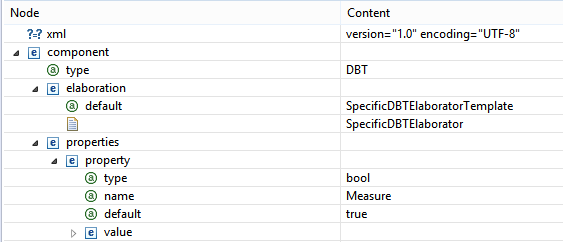
\includegraphics[scale=0.6]{images/mainxml}
}
\caption{DBT xml file.}
\label{fig:dbt_xml} 
\end{figure}

As shown, the user can select the specific behavior for the component (elaboration file) and also change the property defined in the model.




